

\subsection{Overview}
The instruction planner is placed at the top layer of the whole SmartSoft architecture,
therefore it is meant to be the "Swarm Manager" of all Robots that work on a common Task. \\
This approach has been split up into two different aspects, one part of the Instruction planner has to
observe all robots and the states that they are currently in, as well as the task that they are working on.
While the other part of the Instruction planner needs to keep up with the progress on the objective, to
predict and estimate the proximate steps to the goal.

\subsection{Idea}

\begin{figure}[h]
\centering
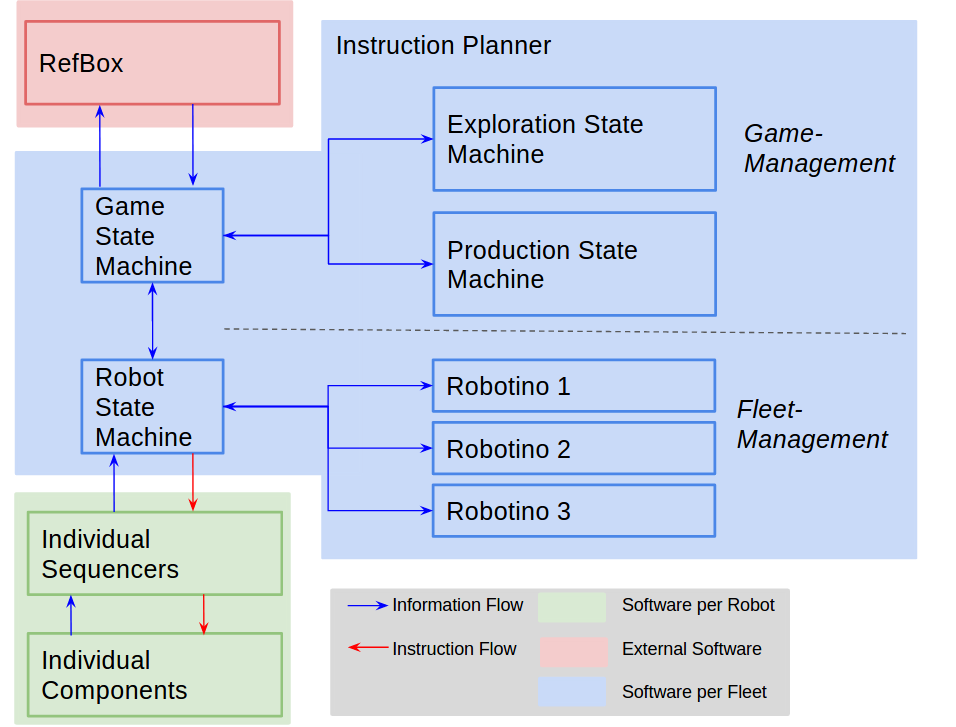
\includegraphics[scale=0.23]{pic/Instructionplanner2018.png}
\caption{Management of Robot Swarm and the Objective}
\label{fig:instr_overview}
\end{figure}

\subsection{Changes}
Previously the architecture, and therefore the purpose of the instruction planner

\subsection{Conclusion}
